\subsection{Jet Energy Resolution}
\label{GBJ2:JER}

The effect from the jet energy resolution (JER) is assessed by smearing the energy in every jet in an event using a Gaussian function with the width given by the measured JER, as described in Section \ref{sec:Det:Jets}, which depends on the jet \pt{} and $\eta$. 
The analysis is then repeated using the smeared jets and the ratio of the final plots were used to see the effect compared to the unsmeared sample.
The smearing procedure is repeated ten times and an average of all curves is the final effect of JER.
This averaging reduced the effect of statistical fluctuations in some bins.
The reconstructed PYTHIA sample is used due to the larger statistics compared to data.
This method assesses the effect of an increase in JER. 
Reducing the JER is not possible, so a symmetric uncertainty band is constructed from the results of the increased JER.

Figures \ref{GBJ2:ResoEnergy:Inclusive_gap} -- \ref{GBJ2:ResoEnergy:Q0} show the ratio of the final distributions from the smeared jets and from the nominal jets.
The different blue histograms represent the 10 implementations of the increased JER, the two red histogram are the uncertainty band found from the average of the blue histograms, and the black points show the PYTHIA statistical uncertainties.  

Figure \ref{GBJ2:ResoEnergy:Inclusive_gap} (a) shows the ratio for the number of events as a function of the dijet rapidity separation, \dy{}.
The effect of the smearing is less than  $1\%$ in all bins.
Figure \ref{GBJ2:ResoEnergy:Inclusive_gap} (b) shows the ratio for the gap fraction as a function of the dijet rapidity separation, \dy{}.
The deviations from unity are very small for low \dy{} and even for large \dy{} are less than  $1\%$.


Figure \ref{GBJ2:ResoEnergy:cos} shows the ratio for \mean{\cosdphi{}} as a function of the dijet rapidity separation, \dy{}, for both (a) inclusive events and (b) gap events.
The JER smearing has a less than  $1\%$ effect on these distributions.
Figure \ref{GBJ2:ResoEnergy:cos2} shows the ratio for \mean{\costwodphi{}} as a function of the dijet rapidity separation, \dy{}, for both (a) inclusive events and (b) gap events.
The effects from the JER smearing are less than  $1\%$ for both the inclusive and gap events.

Figure \ref{GBJ2:ResoEnergy:dphi23} shows the ratio for \dphiDist{} for (a) inclusive events and (b) gap events with  $2<\dy{}<3$.
The effect of the JER smearing is less than  $1\%$ for all bins.
For the lowest \dphi{} bins, the individual ratios of the smeared jets vary by more than at the high \dphi{} bins due to the statistical uncertainty being significantly larger.
Figure \ref{GBJ2:ResoEnergy:dphi45} shows the ratio for \dphiDist{} for (a) inclusive events and (b) gap events with $4<\dy{}<5$.
For both the inclusive and gap events, the effect of the JER smearing is at maximum  $1\%$.
Figure \ref{GBJ2:ResoEnergy:dphi78} shows the ratio for \dphiDist{} for (a) inclusive events and (b) gap events with $7<\dy{}<8$.
For the inclusive events, the effect of the JER smearing is of the order of $2\%$.
For the gap events, the effect of the JER smearing can get large, especially in the low \dphi{} bins. 
Ignoring the two lowest \dphi{} bins, which do not have any data events in them, the uncertainty does not exceed $2\%$.

Figure \ref{GBJ2:ResoEnergy:Q0} shows the ratio for the gap fraction as a function of \qz{} for (a) $2<\dy{}<3$, (b) $4<\dy{}<5$, and (c) $7<\dy{}<8$.
The effect from the smearing is less than $1\%$ in all the ranges.
The spread in the individual smears is larger for more separated dijets due to the increase in statistical uncertainty. 


\begin{figure}
\centering
        \begin{subfigure}[b]{0.5\textwidth}
                \centering
                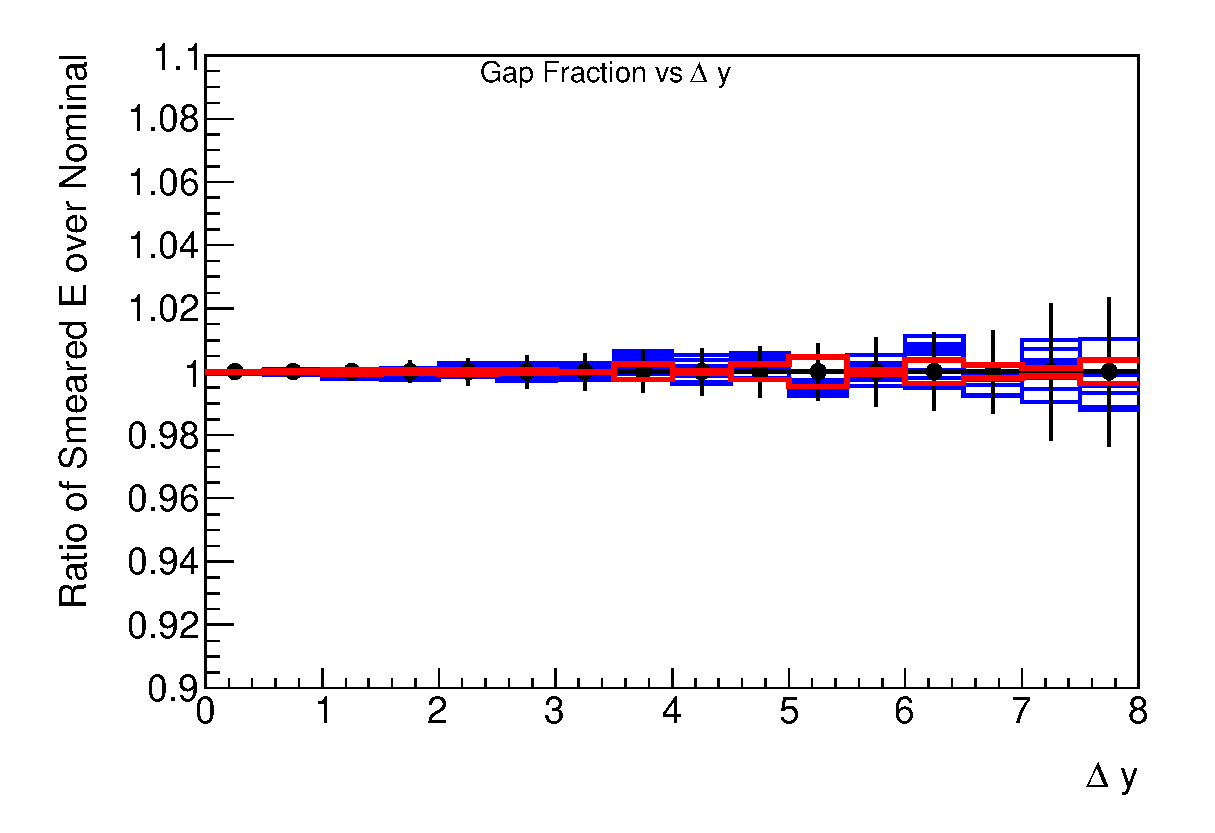
\includegraphics[width=\textwidth]{figures/GBJ2/ResoEnergy/RMS_E___GapFraction_deltaY_Ratio.eps}
        \end{subfigure}%
        \begin{subfigure}[b]{0.5\textwidth}
                \centering
                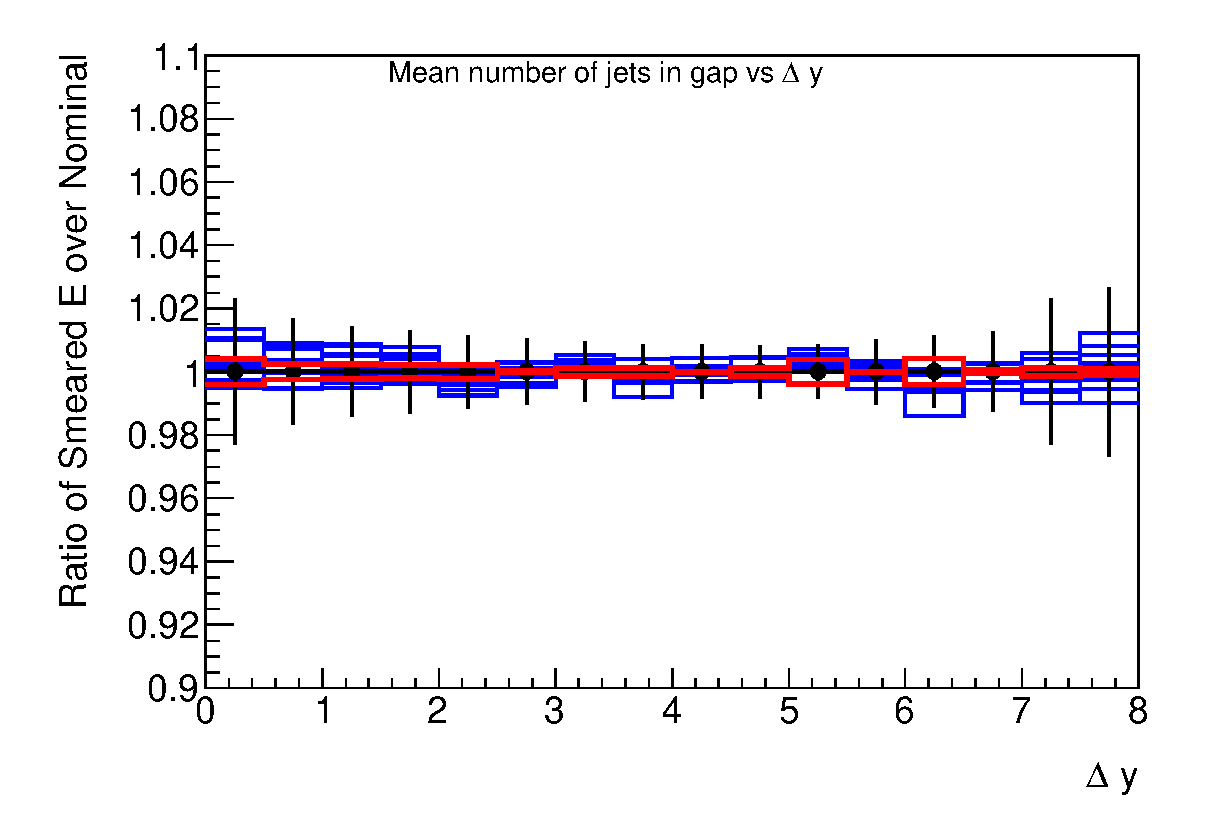
\includegraphics[width=\textwidth]{figures/GBJ2/ResoEnergy/RMS_E___prof_deltaY_njets_Ratio.eps}
        \end{subfigure}%
\caption[Uncertainty bands due to the JER uncertainty for gap fraction and mean number of jets]{
The ratio of (a) the gap fraction and (b) the mean number of jets in the rapidity region between the dijet as a function of $\Delta y$ for reconstructed PYTHIA sample with nominal sample compared to energy smeared sample.
\label{GBJ2:ResoEnergy:Inclusive_gap}}
\end{figure}

\begin{figure}
\centering
        \begin{subfigure}[b]{0.5\textwidth}
                \centering
                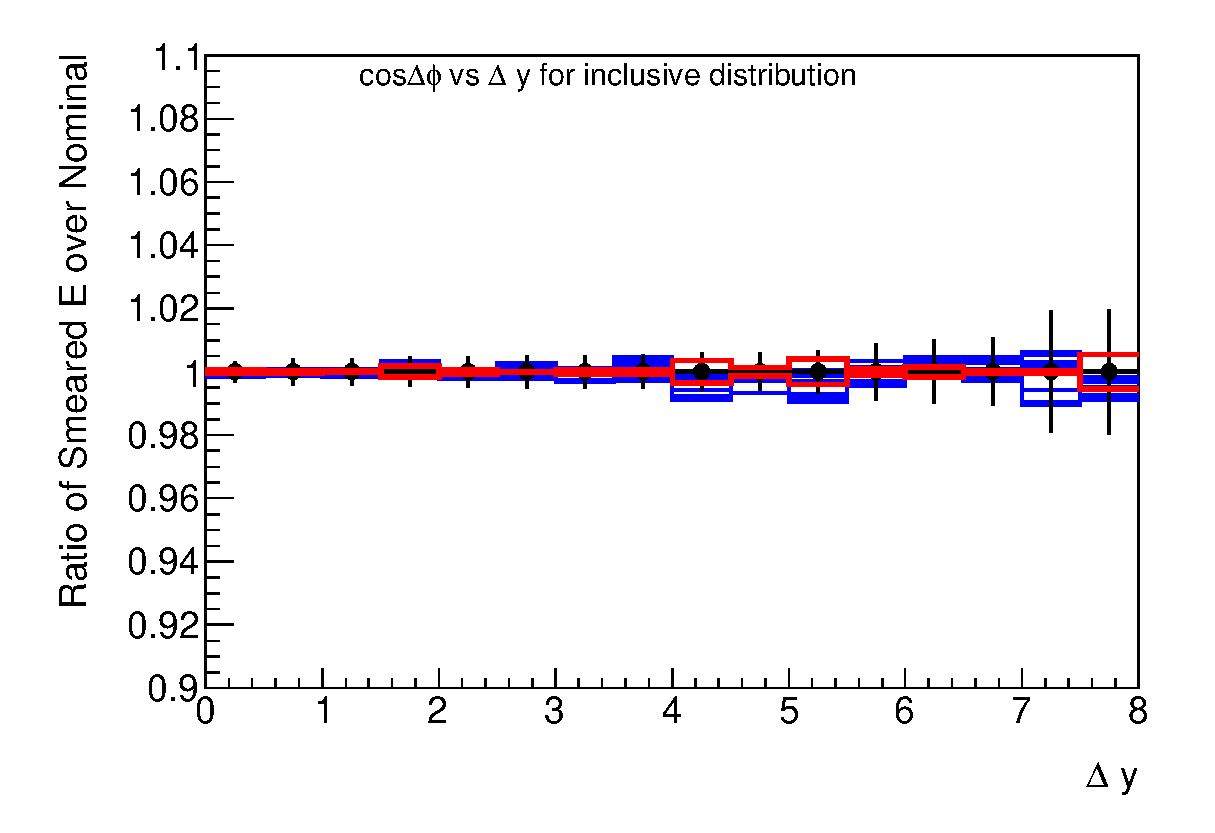
\includegraphics[width=\textwidth]{figures/GBJ2/ResoEnergy/RMS_E___cosdPhi_deltaY_Ratio.eps}
        \end{subfigure}%
        \begin{subfigure}[b]{0.5\textwidth}
                \centering
                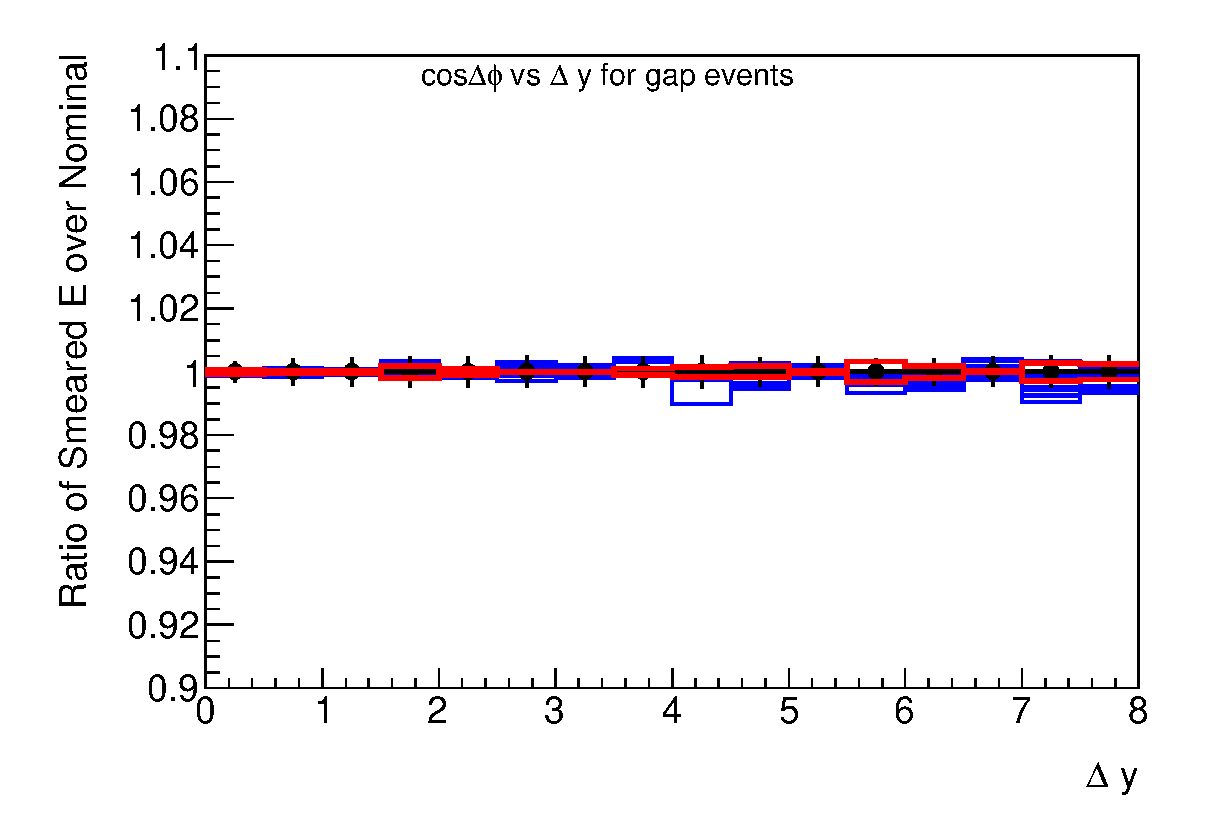
\includegraphics[width=\textwidth]{figures/GBJ2/ResoEnergy/RMS_E___cosdPhi_deltaY_gap_Ratio.eps}
        \end{subfigure}%
\caption[Uncertainty bands due to the JER uncertainty for \mean{\cosdphi{}}]{
The ratio of \mean{\cosdphi{}} as a function of \dy{} for (a) inclusive and (b) gap events reconstructed PYTHIA sample with nominal sample compared to energy smeared sample.
\label{GBJ2:ResoEnergy:cos}}
\end{figure}

\begin{figure}
\centering
        \begin{subfigure}[b]{0.5\textwidth}
                \centering
                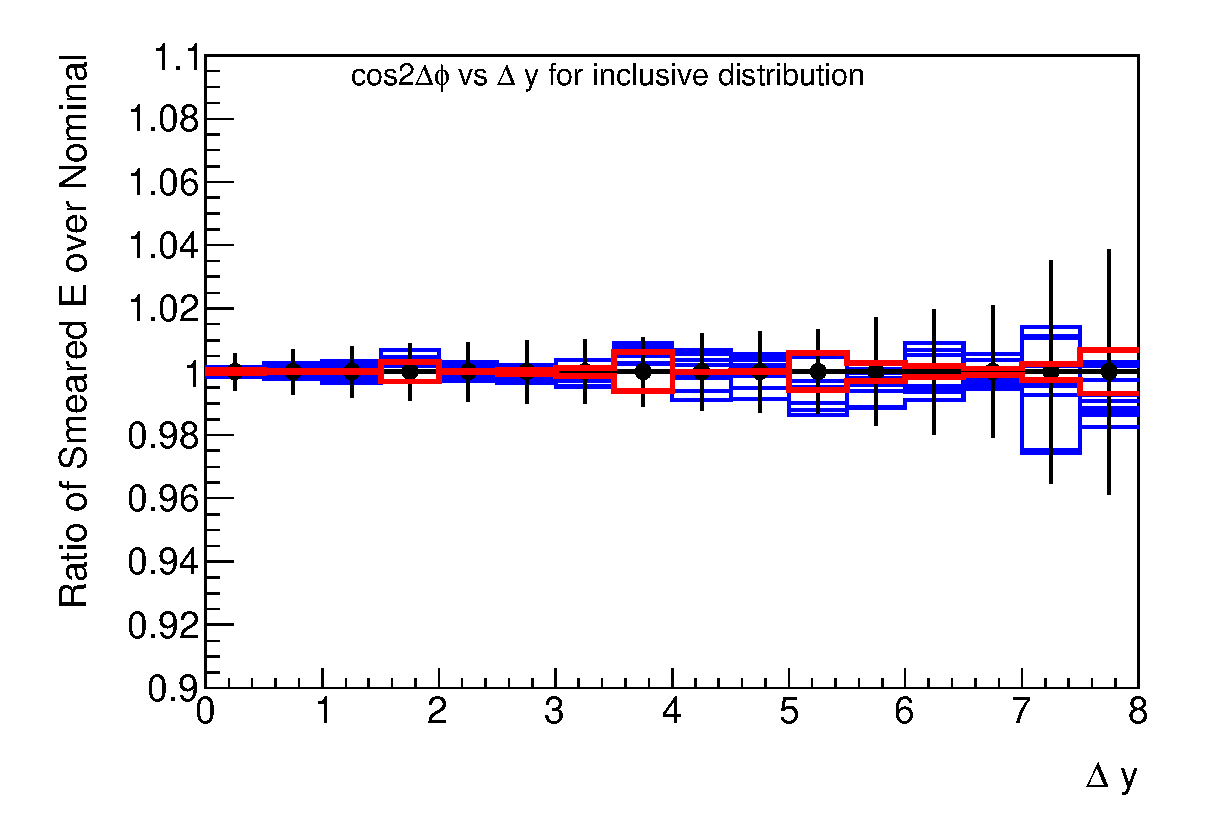
\includegraphics[width=\textwidth]{figures/GBJ2/ResoEnergy/RMS_E___cos2dPhi_deltaY_Ratio.eps}
        \end{subfigure}%
        \begin{subfigure}[b]{0.5\textwidth}
                \centering
                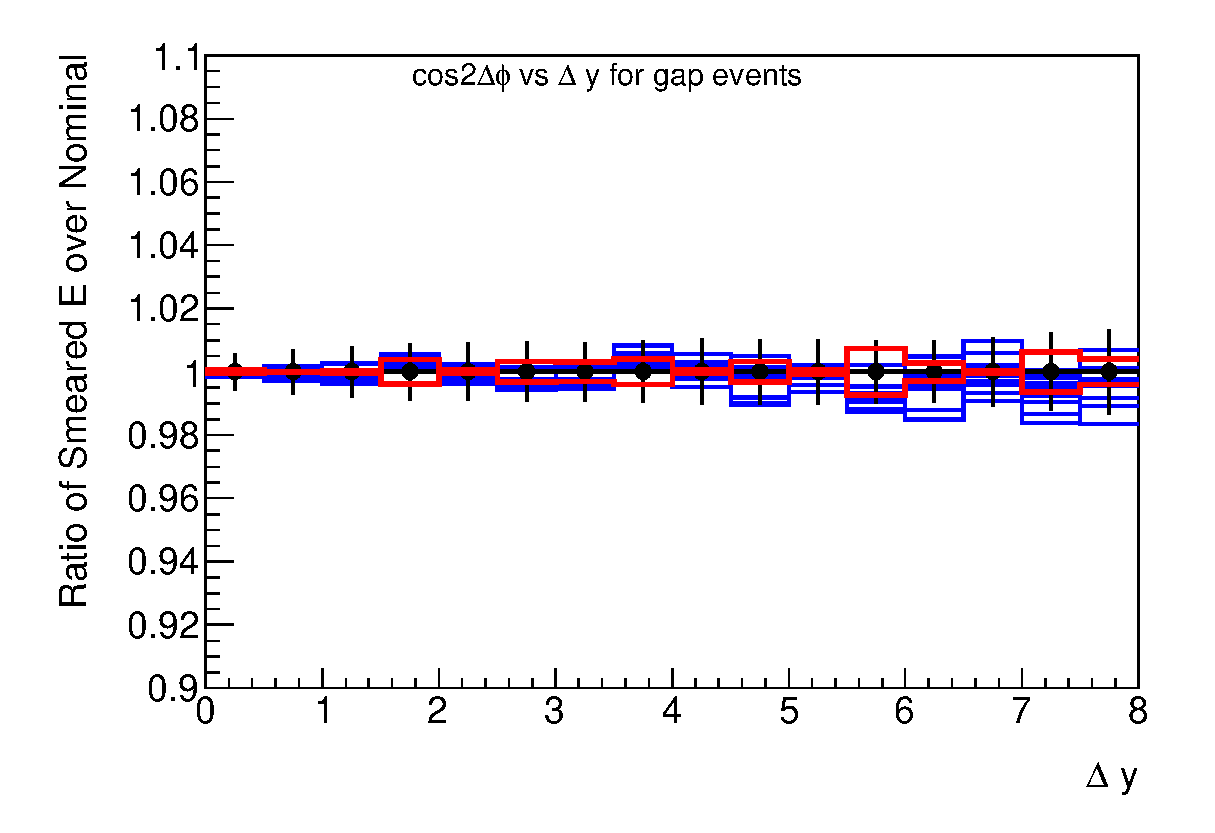
\includegraphics[width=\textwidth]{figures/GBJ2/ResoEnergy/RMS_E___cos2dPhi_deltaY_gap_Ratio.eps}
        \end{subfigure}%
\caption[Uncertainty bands due to the JER uncertainty for \mean{\costwodphi{}}]{
The ratio of \mean{\costwodphi{}} as a function of \dy{} for (a) inclusive and (b) gap events reconstructed PYTHIA sample with nominal sample compared to energy smeared sample.
\label{GBJ2:ResoEnergy:cos2}}
\end{figure}

\begin{figure}
\centering
        \begin{subfigure}[b]{0.5\textwidth}
                \centering
                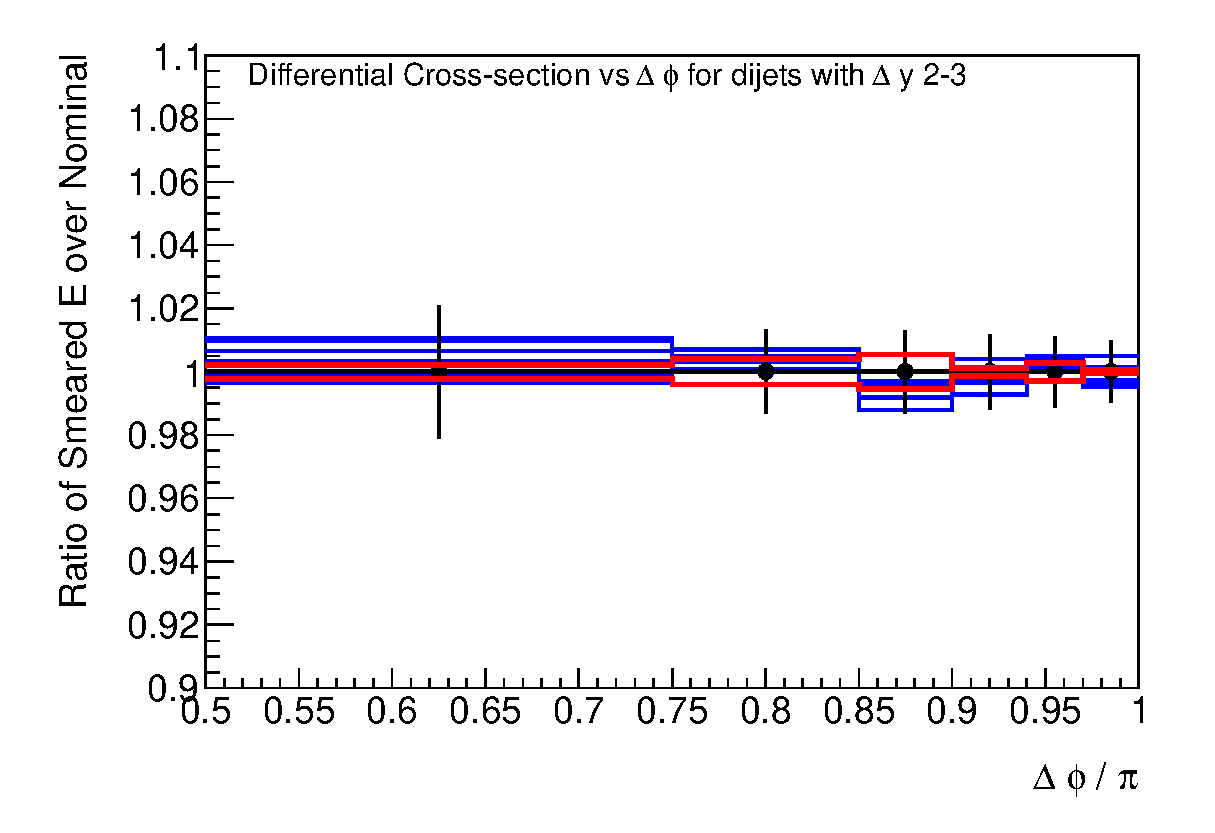
\includegraphics[width=\textwidth]{figures/GBJ2/ResoEnergy/RMS_E___dPhi__2_3_Ratio.eps}
        \end{subfigure}%
        \begin{subfigure}[b]{0.5\textwidth}
                \centering
                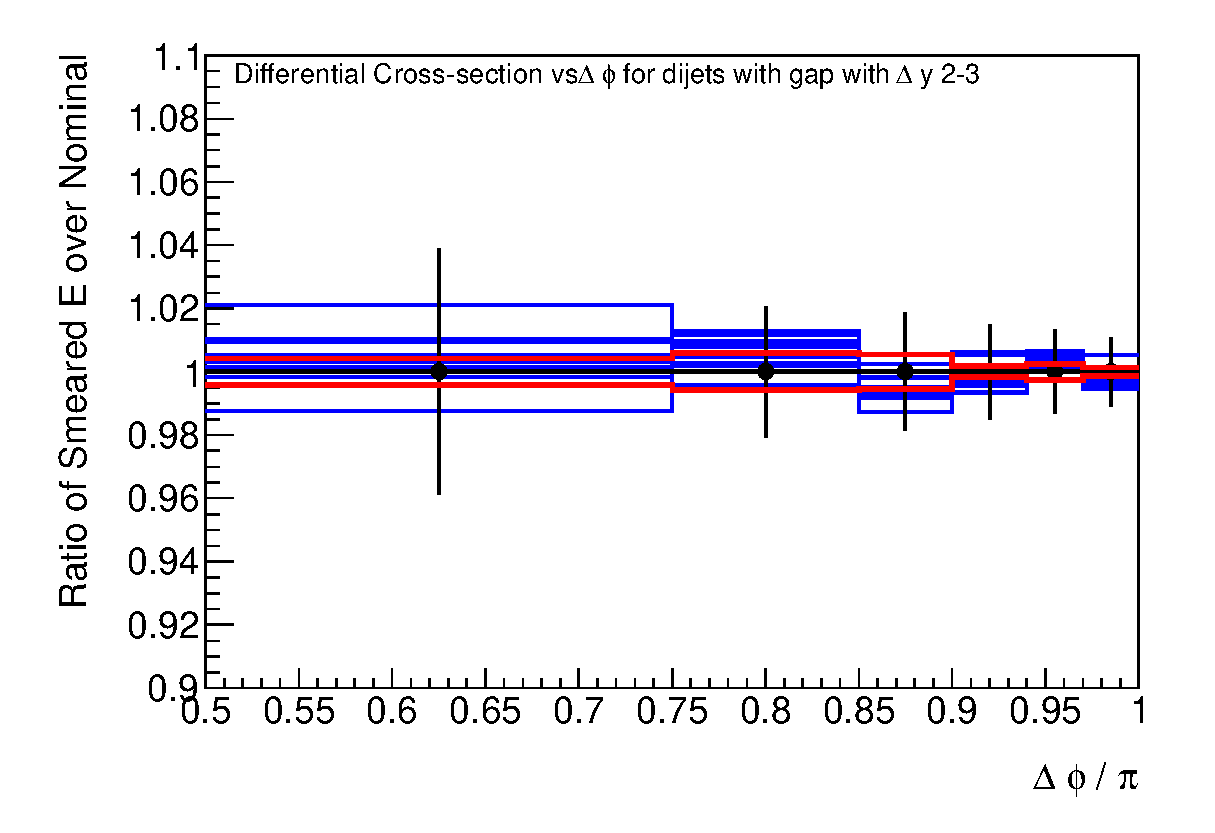
\includegraphics[width=\textwidth]{figures/GBJ2/ResoEnergy/RMS_E___dPhi_gap__2_3_Ratio.eps}
        \end{subfigure}%

        \begin{subfigure}[b]{0.5\textwidth}
                \centering
                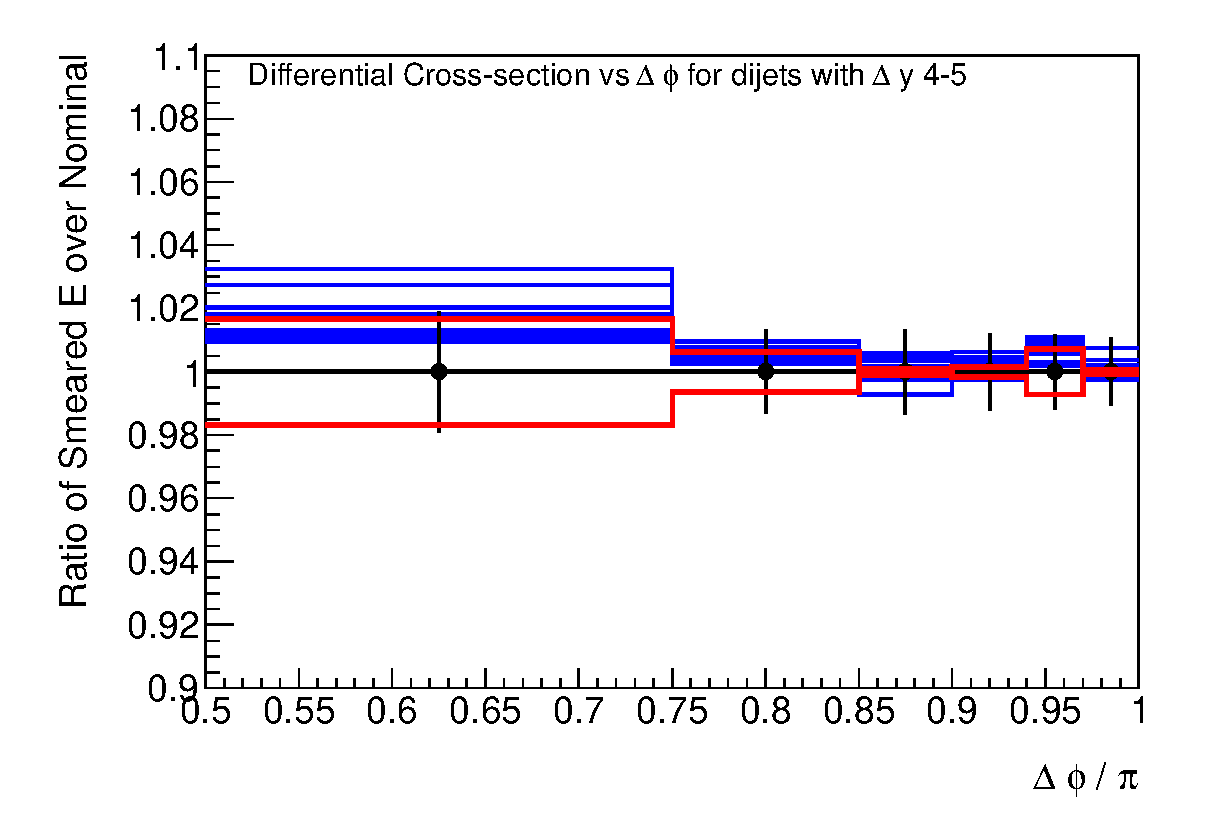
\includegraphics[width=\textwidth]{figures/GBJ2/ResoEnergy/RMS_E___dPhi__4_5_Ratio.eps}
        \end{subfigure}%
        \begin{subfigure}[b]{0.5\textwidth}
                \centering
                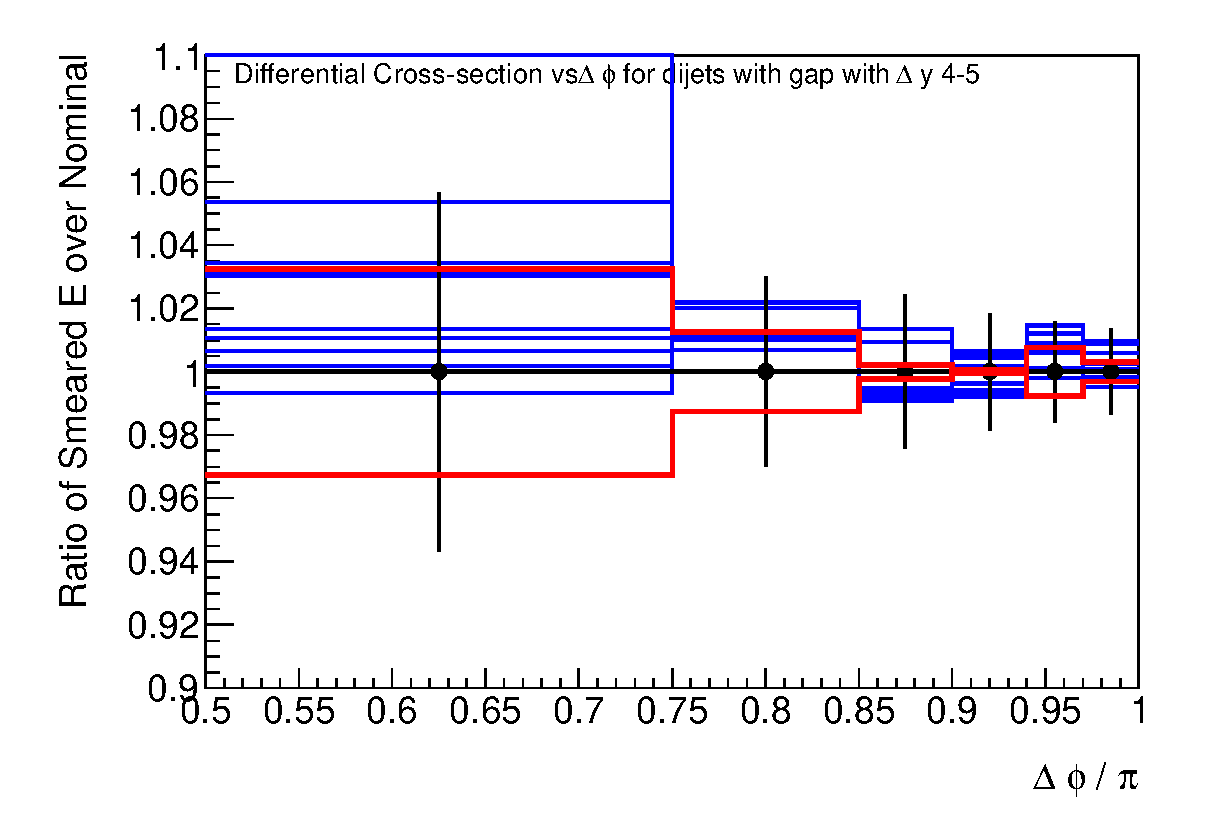
\includegraphics[width=\textwidth]{figures/GBJ2/ResoEnergy/RMS_E___dPhi_gap__4_5_Ratio.eps}
        \end{subfigure}%

        \begin{subfigure}[b]{0.5\textwidth}
                \centering
                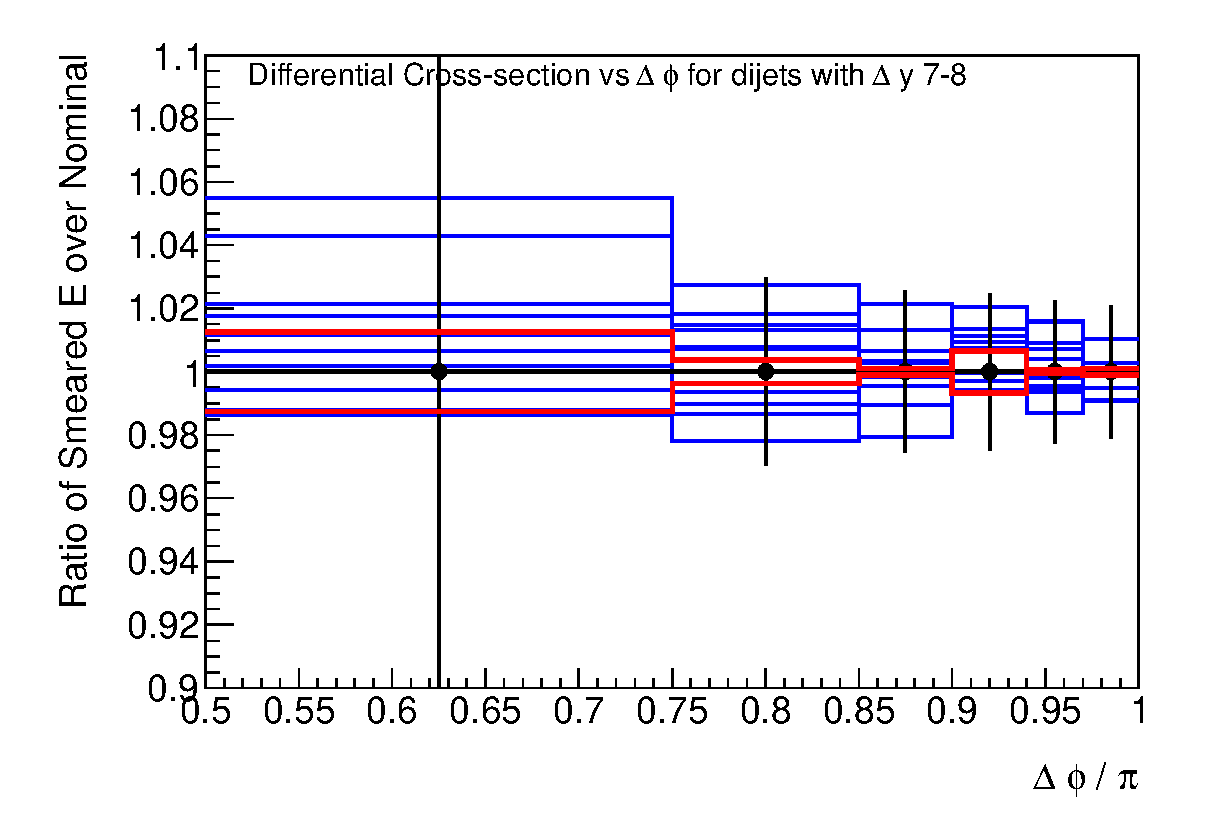
\includegraphics[width=\textwidth]{figures/GBJ2/ResoEnergy/RMS_E___dPhi__7_8_Ratio.eps}
        \end{subfigure}%
        \begin{subfigure}[b]{0.5\textwidth}
                \centering
                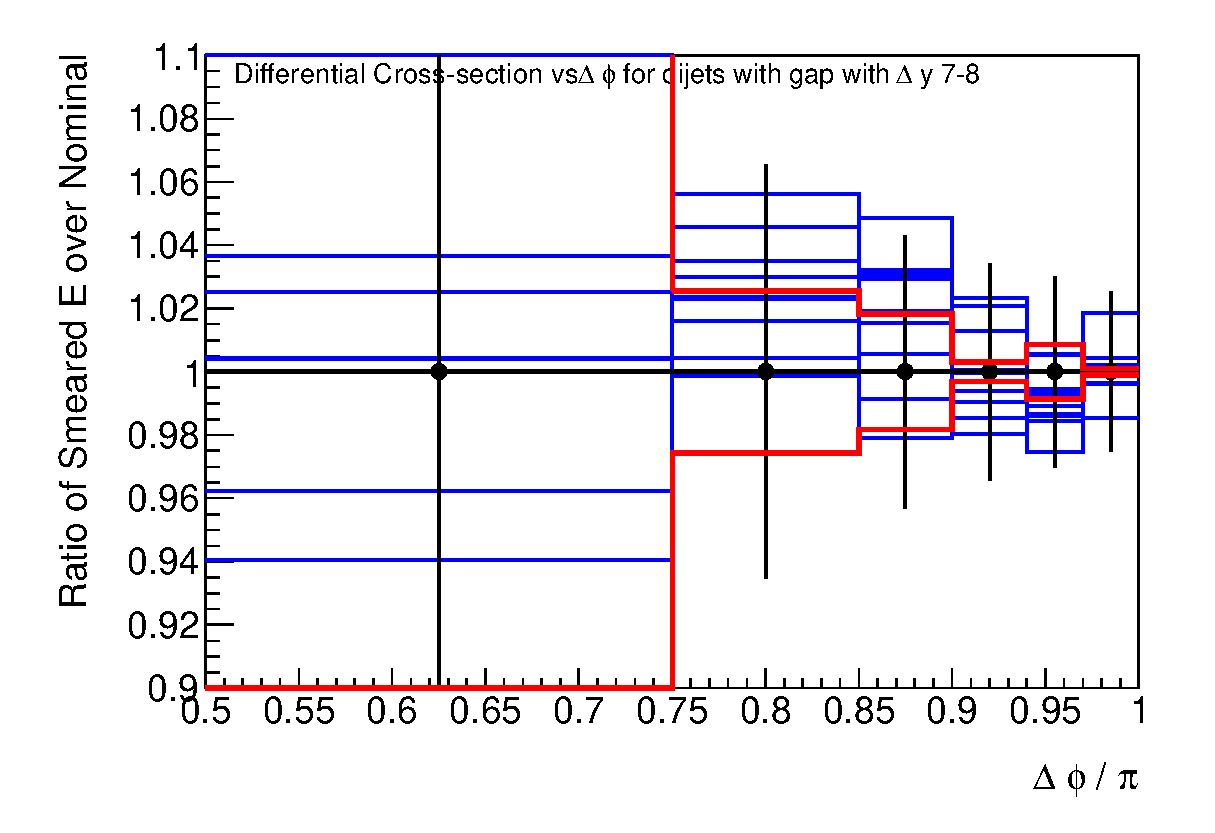
\includegraphics[width=\textwidth]{figures/GBJ2/ResoEnergy/RMS_E___dPhi_gap__7_8_Ratio.eps}
        \end{subfigure}%
\caption[Uncertainty bands due to the JER uncertainty for \dphiDist{} for $7<\dy{}<8$]{
The ratio of \dphiDist{} for $7<\dy{}<8$ for (a) inclusive and (b) gap events reconstructed PYTHIA sample with nominal sample compared to energy smeared sample.
\label{GBJ2:ResoEnergy:dphi78}}
\end{figure}


\begin{figure}
\centering
        \begin{subfigure}[b]{0.5\textwidth}
                \centering
                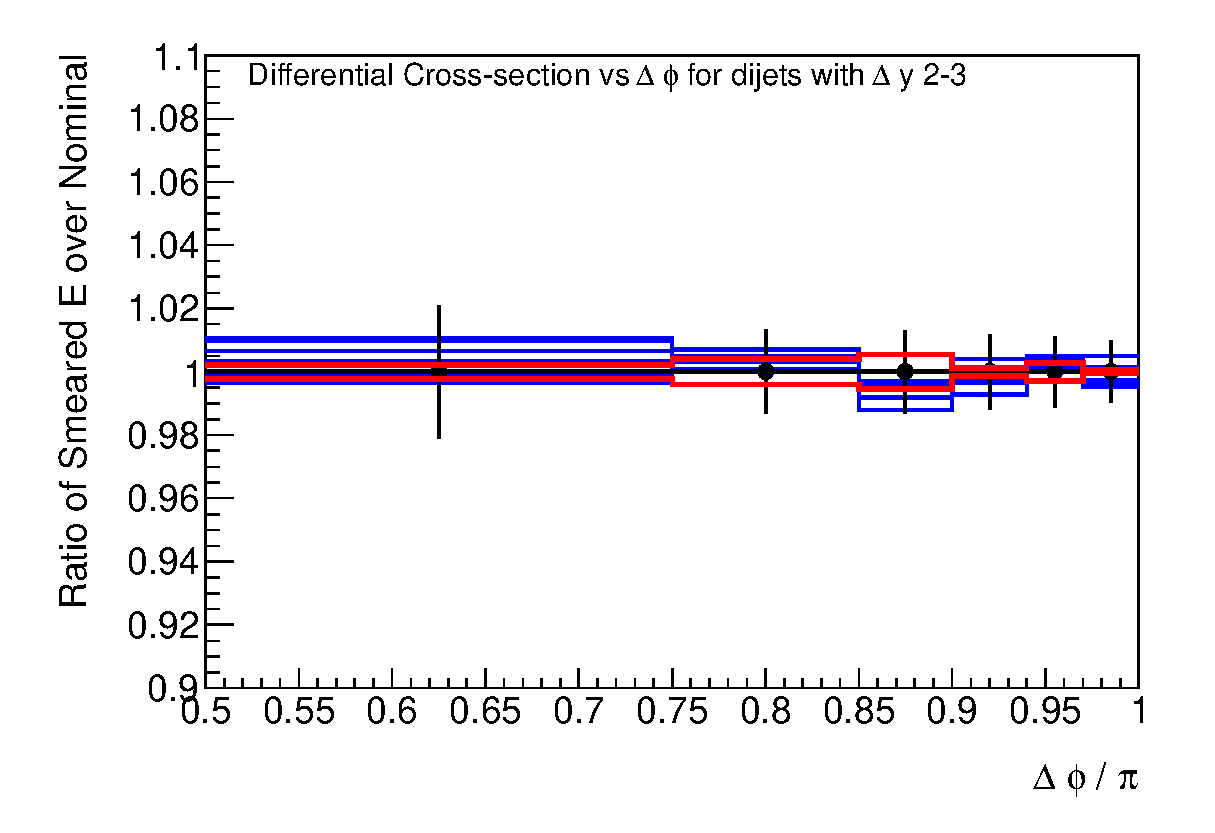
\includegraphics[width=\textwidth]{figures/GBJ2/ResoEnergy/RMS_E___dPhi__2_3_Ratio.eps}
        \end{subfigure}%
        \begin{subfigure}[b]{0.5\textwidth}
                \centering
                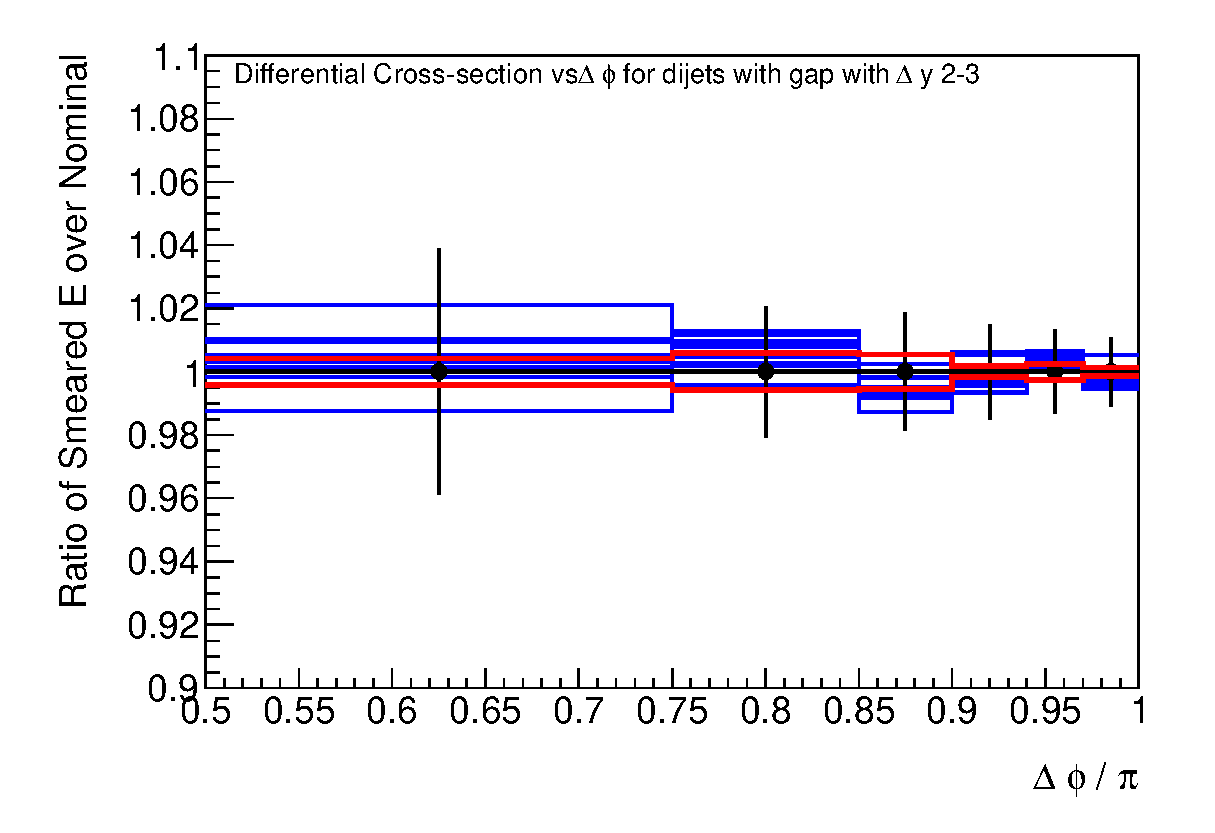
\includegraphics[width=\textwidth]{figures/GBJ2/ResoEnergy/RMS_E___dPhi_gap__2_3_Ratio.eps}
        \end{subfigure}%
\caption[Uncertainty bands due to the JER uncertainty for \dphiDist{} for $2<\dy{}<3$]{
The ratio of \dphiDist{} for $2<\dy{}<3$ for (a) inclusive and (b) gap events reconstructed PYTHIA sample with nominal sample compared to energy smeared sample.
\label{GBJ2:ResoEnergy:dphi23}}
\end{figure}


\begin{figure}
\centering
        \begin{subfigure}[b]{0.5\textwidth}
                \centering
                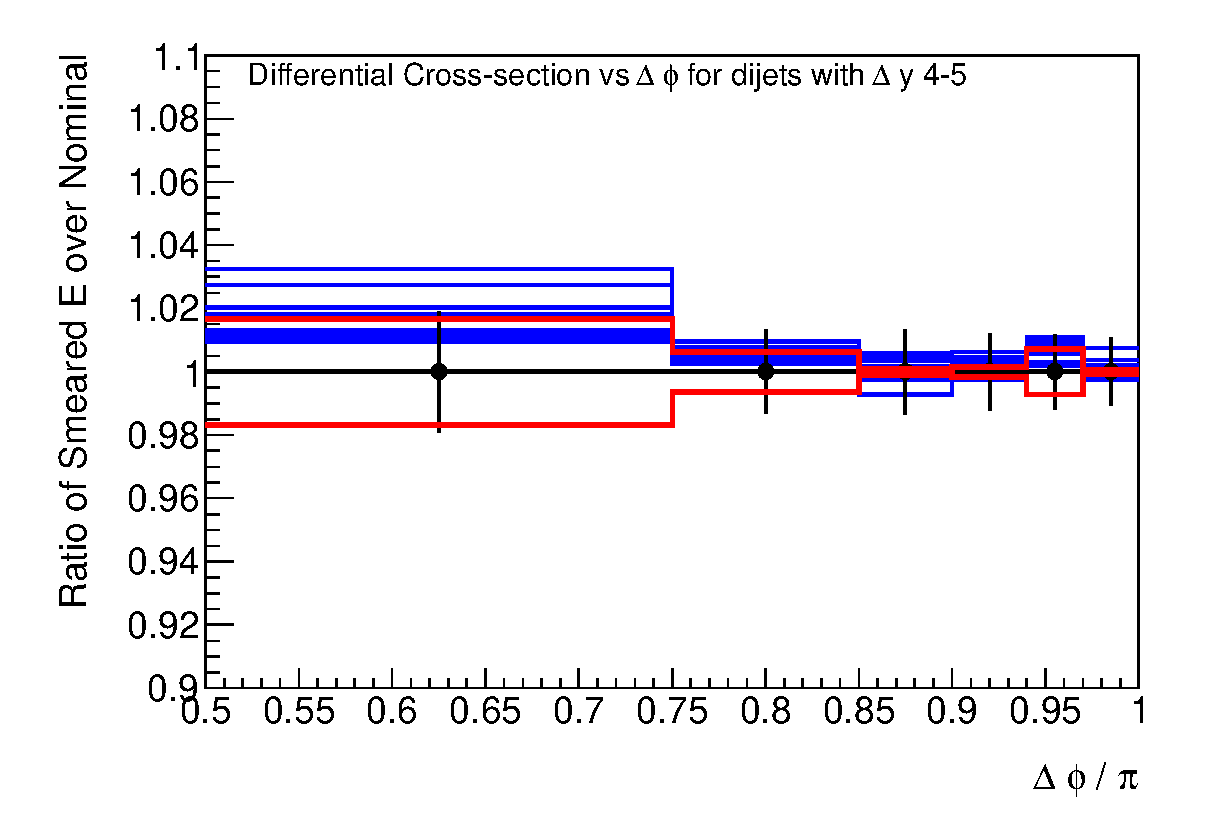
\includegraphics[width=\textwidth]{figures/GBJ2/ResoEnergy/RMS_E___dPhi__4_5_Ratio.eps}
        \end{subfigure}%
        \begin{subfigure}[b]{0.5\textwidth}
                \centering
                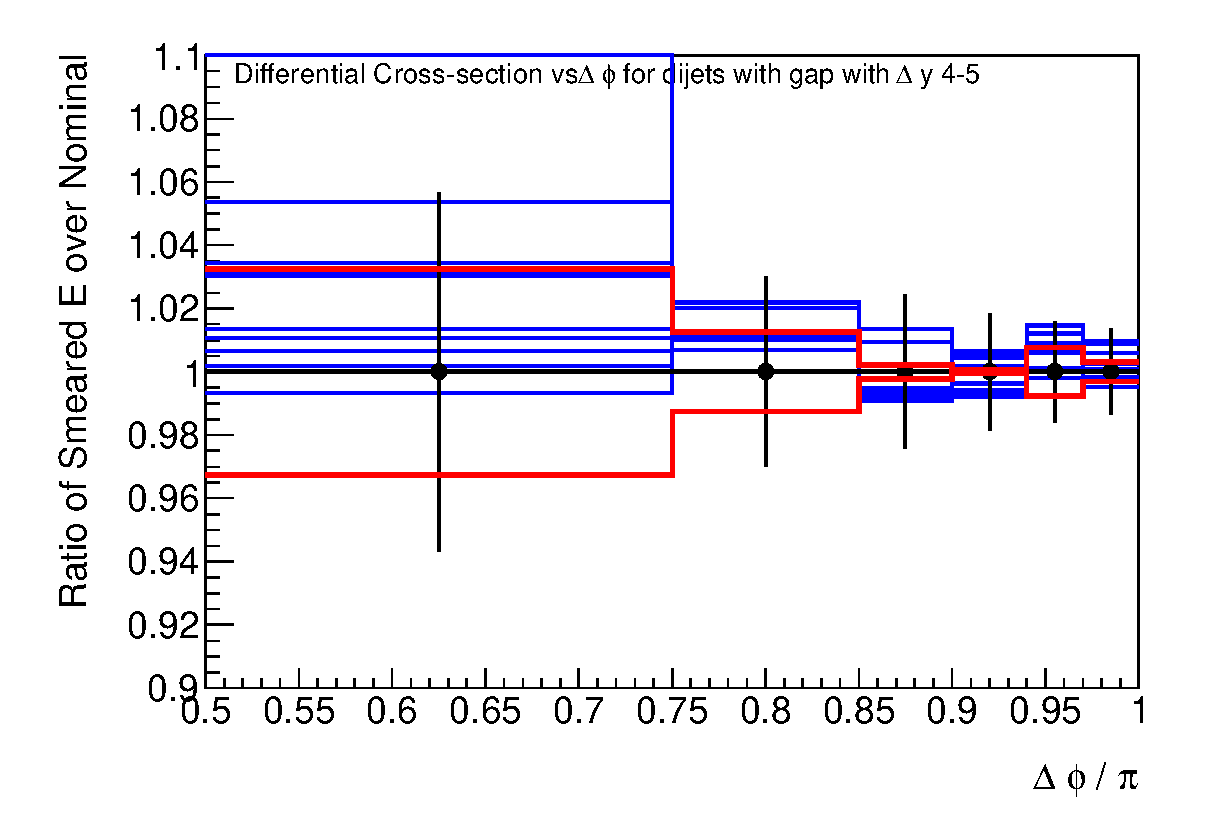
\includegraphics[width=\textwidth]{figures/GBJ2/ResoEnergy/RMS_E___dPhi_gap__4_5_Ratio.eps}
        \end{subfigure}%
\caption[Uncertainty bands due to the JER uncertainty for \dphiDist{} for $4<\dy{}<5$]{
The ratio of \dphiDist{} for $4<\dy{}<5$ for (a) inclusive and (b) gap events reconstructed PYTHIA sample with nominal sample compared to energy smeared sample.
\label{GBJ2:ResoEnergy:dphi45}}
\end{figure}



\begin{figure}
\centering
        \begin{subfigure}[b]{0.5\textwidth}
                \centering
                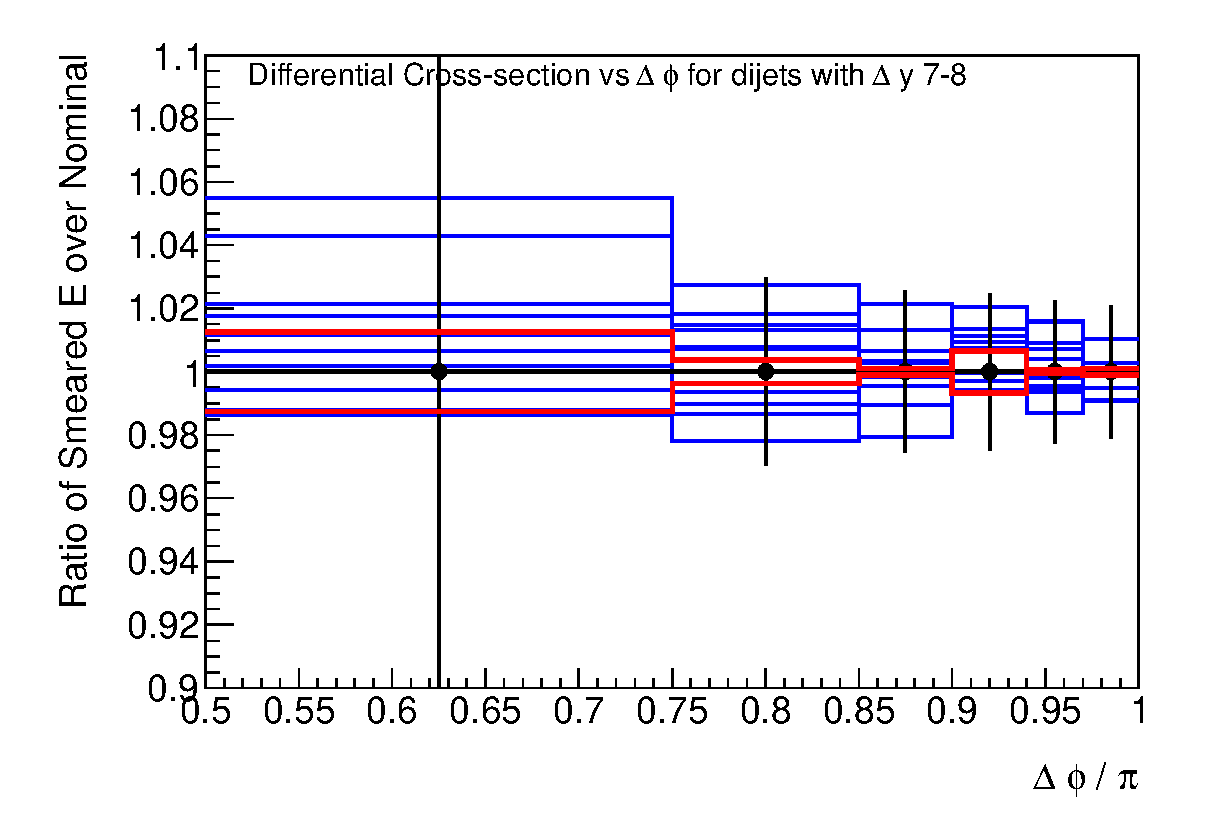
\includegraphics[width=\textwidth]{figures/GBJ2/ResoEnergy/RMS_E___dPhi__7_8_Ratio.eps}
        \end{subfigure}%
        \begin{subfigure}[b]{0.5\textwidth}
                \centering
                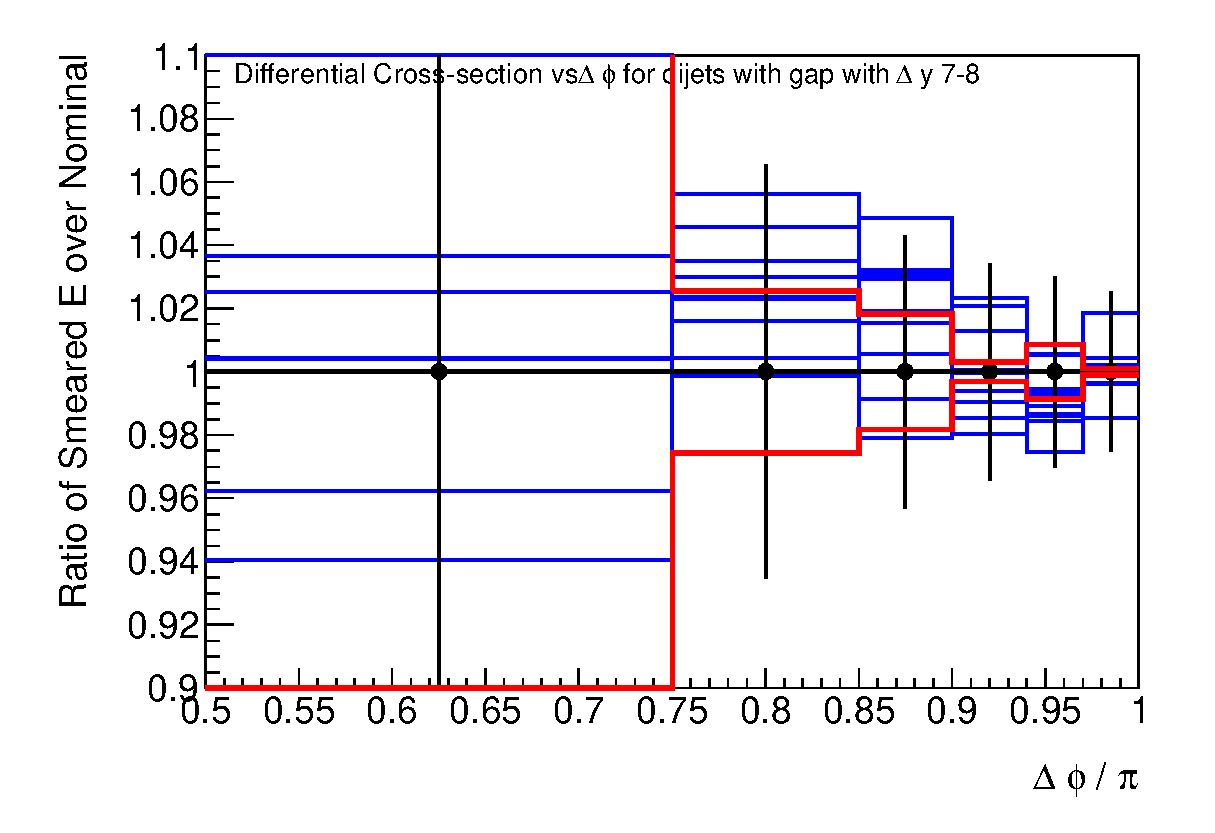
\includegraphics[width=\textwidth]{figures/GBJ2/ResoEnergy/RMS_E___dPhi_gap__7_8_Ratio.eps}
        \end{subfigure}%
\caption[Uncertainty bands due to the JER uncertainty for \dphiDist{} for $7<\dy{}<8$]{
The ratio of \dphiDist{} for $7<\dy{}<8$ for (a) inclusive and (b) gap events reconstructed PYTHIA sample with nominal sample compared to energy smeared sample.
\label{GBJ2:ResoEnergy:dphi78}}
\end{figure}


\begin{figure}
\centering
\mbox{
        \begin{subfigure}[b]{0.33\textwidth}
                \centering
                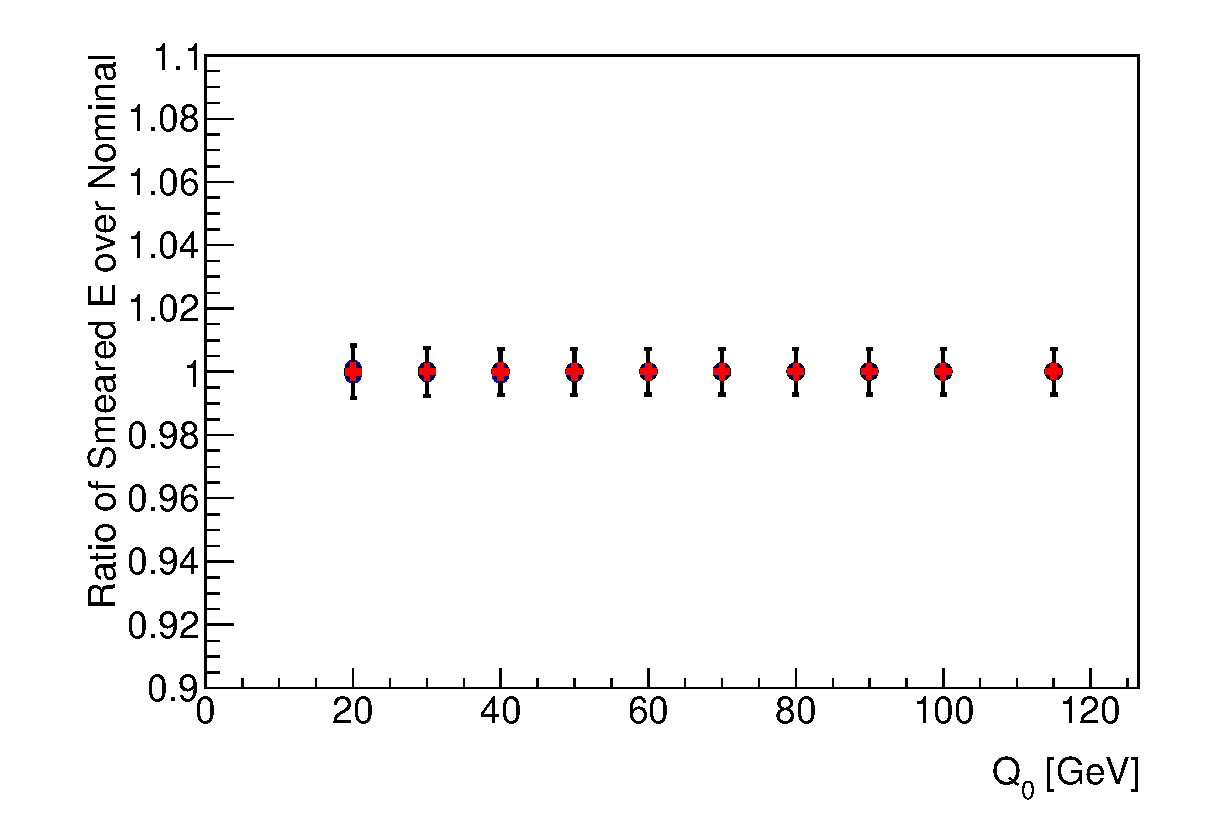
\includegraphics[width=\textwidth]{figures/GBJ2/ResoEnergy/RMS_E_2_3__Q0_Ratio.eps}
        \end{subfigure}%
        \begin{subfigure}[b]{0.33\textwidth}
                \centering
                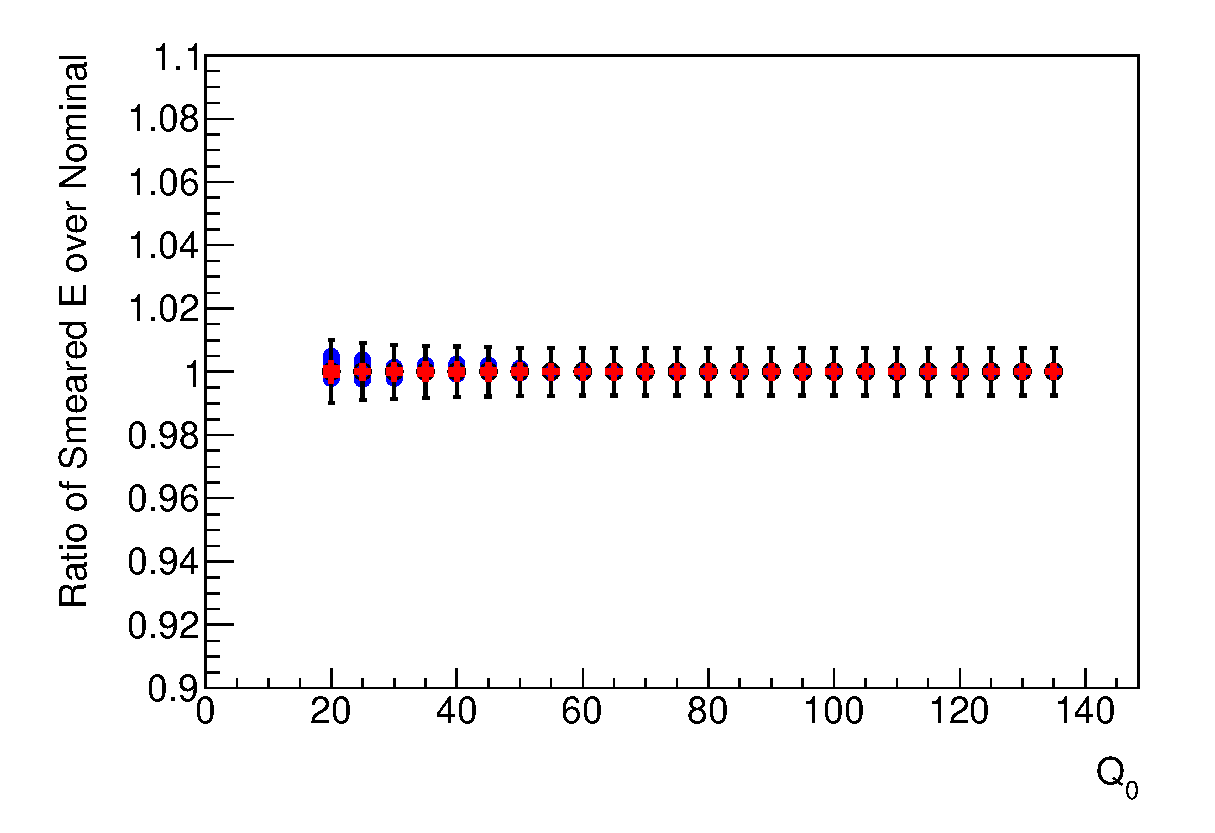
\includegraphics[width=\textwidth]{figures/GBJ2/ResoEnergy/RMS_E_4_5__Q0_Ratio.eps}
        \end{subfigure}%
        \begin{subfigure}[b]{0.33\textwidth}
                \centering
                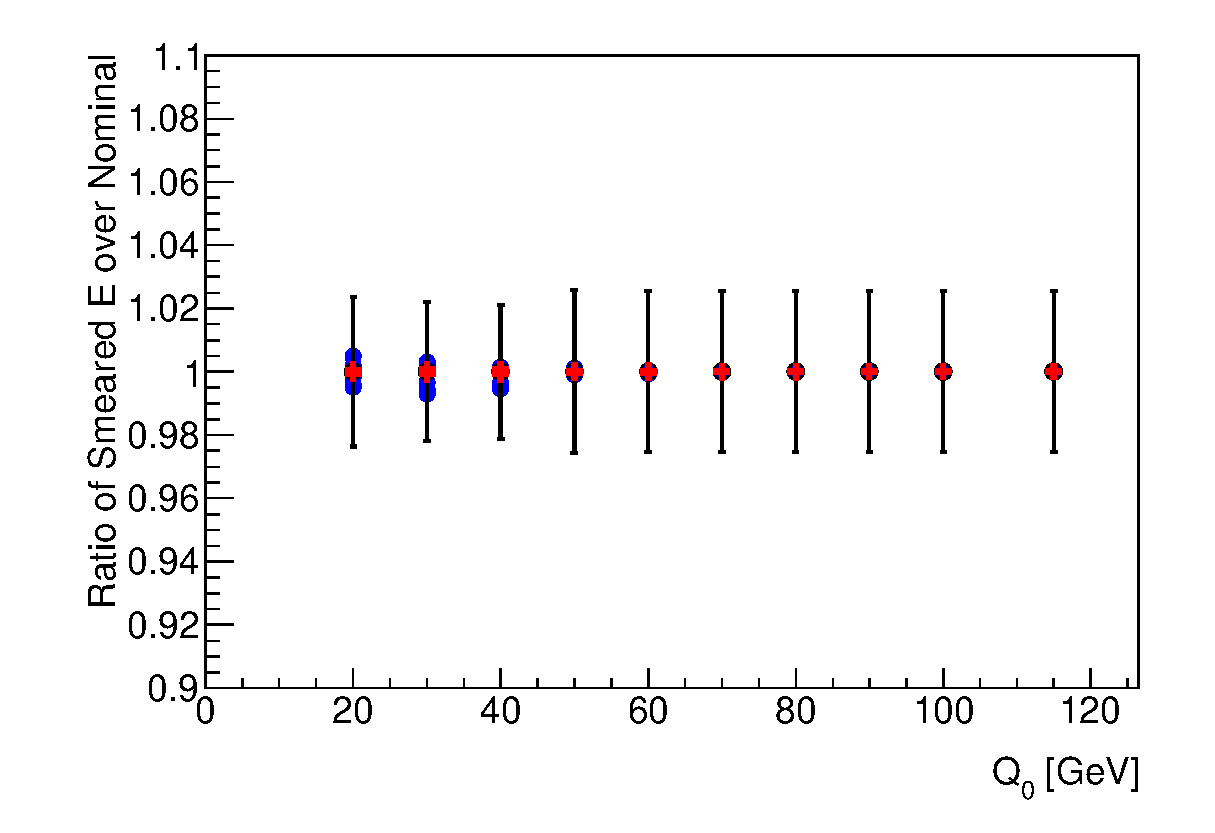
\includegraphics[width=\textwidth]{figures/GBJ2/ResoEnergy/RMS_E_7_8__Q0_Ratio.eps}
        \end{subfigure}%
                              }
\caption[Uncertainty bands due to the JER uncertainty for gap fraction as a function of \qz{}]{
The gap fraction as a function of \qz{} for dijet events with (a) $2<\dy{}<3$, (b) $4<\dy{}<5$, and (c) $7<\dy{}<8$,  for reconstructed PYTHIA sample with nominal sample compared to energy smeared sample.
\label{GBJ2:ResoEnergy:Q0}}
\end{figure}



